\section{Повторение электрофореза (16 сентября)}

Весь электрофорез был повторен с новыми белками-маркерами (\ref{ef}).

\subsection{Маркеры для электрофореза: SM0671}
\begin{enumerate}
\item 170 kDa
\item 130 kDa
\item 95 kDa
\item 72 kDa -- красный
\item 55 kDa
\item 43 kDa
\item 34 kDa
\item 26 kDa
\item 17 kDa
\item 10 kDa -- желтый
\end{enumerate}

\subsection{Проведение электрофореза}
В 10 лунок геля были нанесены образцы:
\begin{enumerate}
\item маркер
\item проба 1 (8 µl, 4 µg)
\item проба 2 (8 µl, 4 µg)
\item проба 3 (8 µl, 4 µg)
\item проба 4 (8 µl, 4 µg)
\item пустая
\item маркер
\end{enumerate}

% FIXME Параметры электрофореза (сила тока и напряжение)

\subsection{Результаты электрофореза}
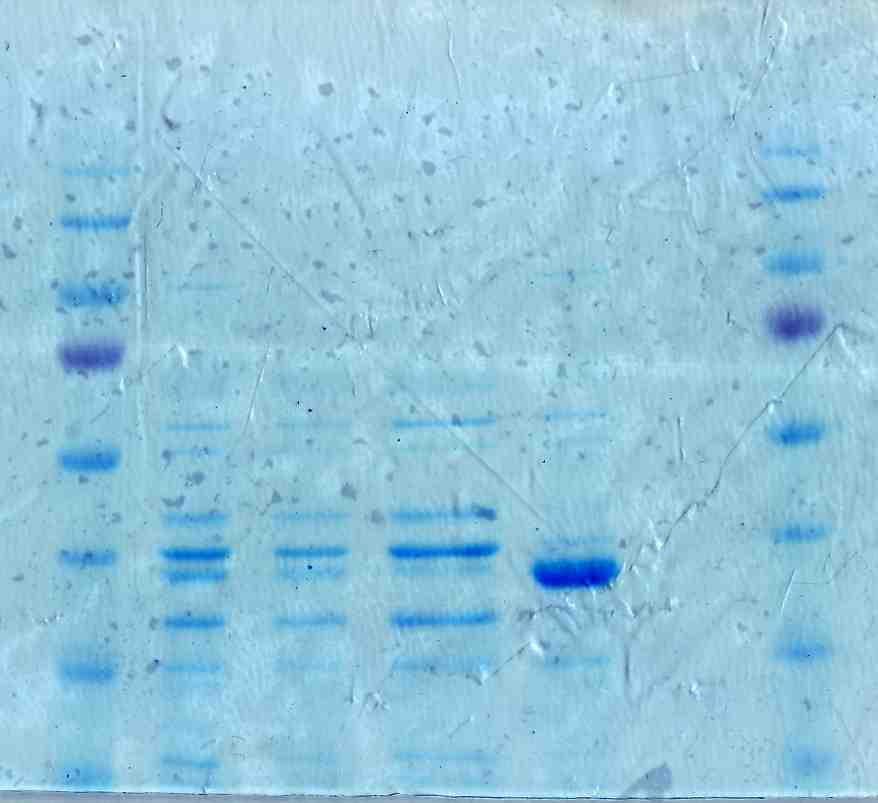
\includegraphics[height=0.3\textheight]{ef-2.jpg}

\subsection{Вычисление массы выделенного белка}
Выделенный белок немного легче маркера 6, имеющего массу 43 kDa.
Это согласуется с литературными данными (см. \ref{lit-m}).

